\documentclass{standalone}
\makeatletter\AtBeginDocument{\@buildstepset{1,2,3,4}}\makeatother
\usepackage{tikz}
\usetikzlibrary{intersections, calc}
\usepackage{hsbcommon}
\begin{document}
    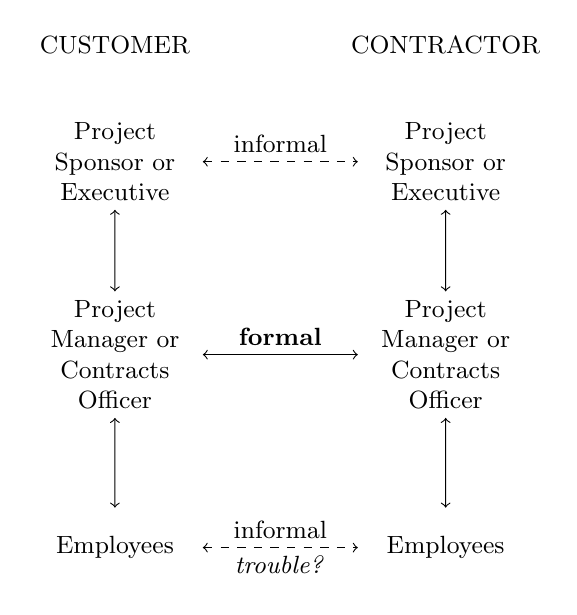
\begin{tikzpicture}[scale=0.7]\small
        \def\myx{3}
        \def\myy{3.5}
        \node       at (-\myx,\myy+5.5cm) {CUSTOMER};
        \node       at (\myx,\myy+5.5cm) {CONTRACTOR};
        \node[text width=2cm, align=center, minimum height=1cm] (sp1) at (-\myx,\myy) {Project Sponsor or Executive};
        \node[text width=2cm, align=center, minimum height=1cm] (pm1) at (-\myx,0) {Project Manager or Contracts Officer};
        \node[text width=2cm, align=center, minimum height=1cm] (em1) at (-\myx,-\myy) {Employees};

        \node[text width=2cm, align=center, minimum height=1cm] (sp2) at (\myx,\myy) {Project Sponsor or Executive};
        \node[text width=2cm, align=center, minimum height=1cm] (pm2) at (\myx,0) {Project Manager or Contracts Officer};
        \node[text width=2cm, align=center, minimum height=1cm] (em2) at (\myx,-\myy) {Employees};

        \draw[<->] (sp1) -- (pm1);
        \draw[<->] (pm1) -- (em1);

        \draw[<->] (sp2) -- (pm2);
        \draw[<->] (pm2) -- (em2);

        \draw[<->,dashed] (sp1) -- node[above] {informal} (sp2) ;
        \draw[<->] (pm1) -- node[above] {\textbf{formal}} (pm2) ;
        \draw[<->,dashed] (em1) -- node[above] {informal} node[below] {\emph{trouble?}} (em2) ;
    \end{tikzpicture}
\end{document}
